\begin{figure}[htb]
\centering
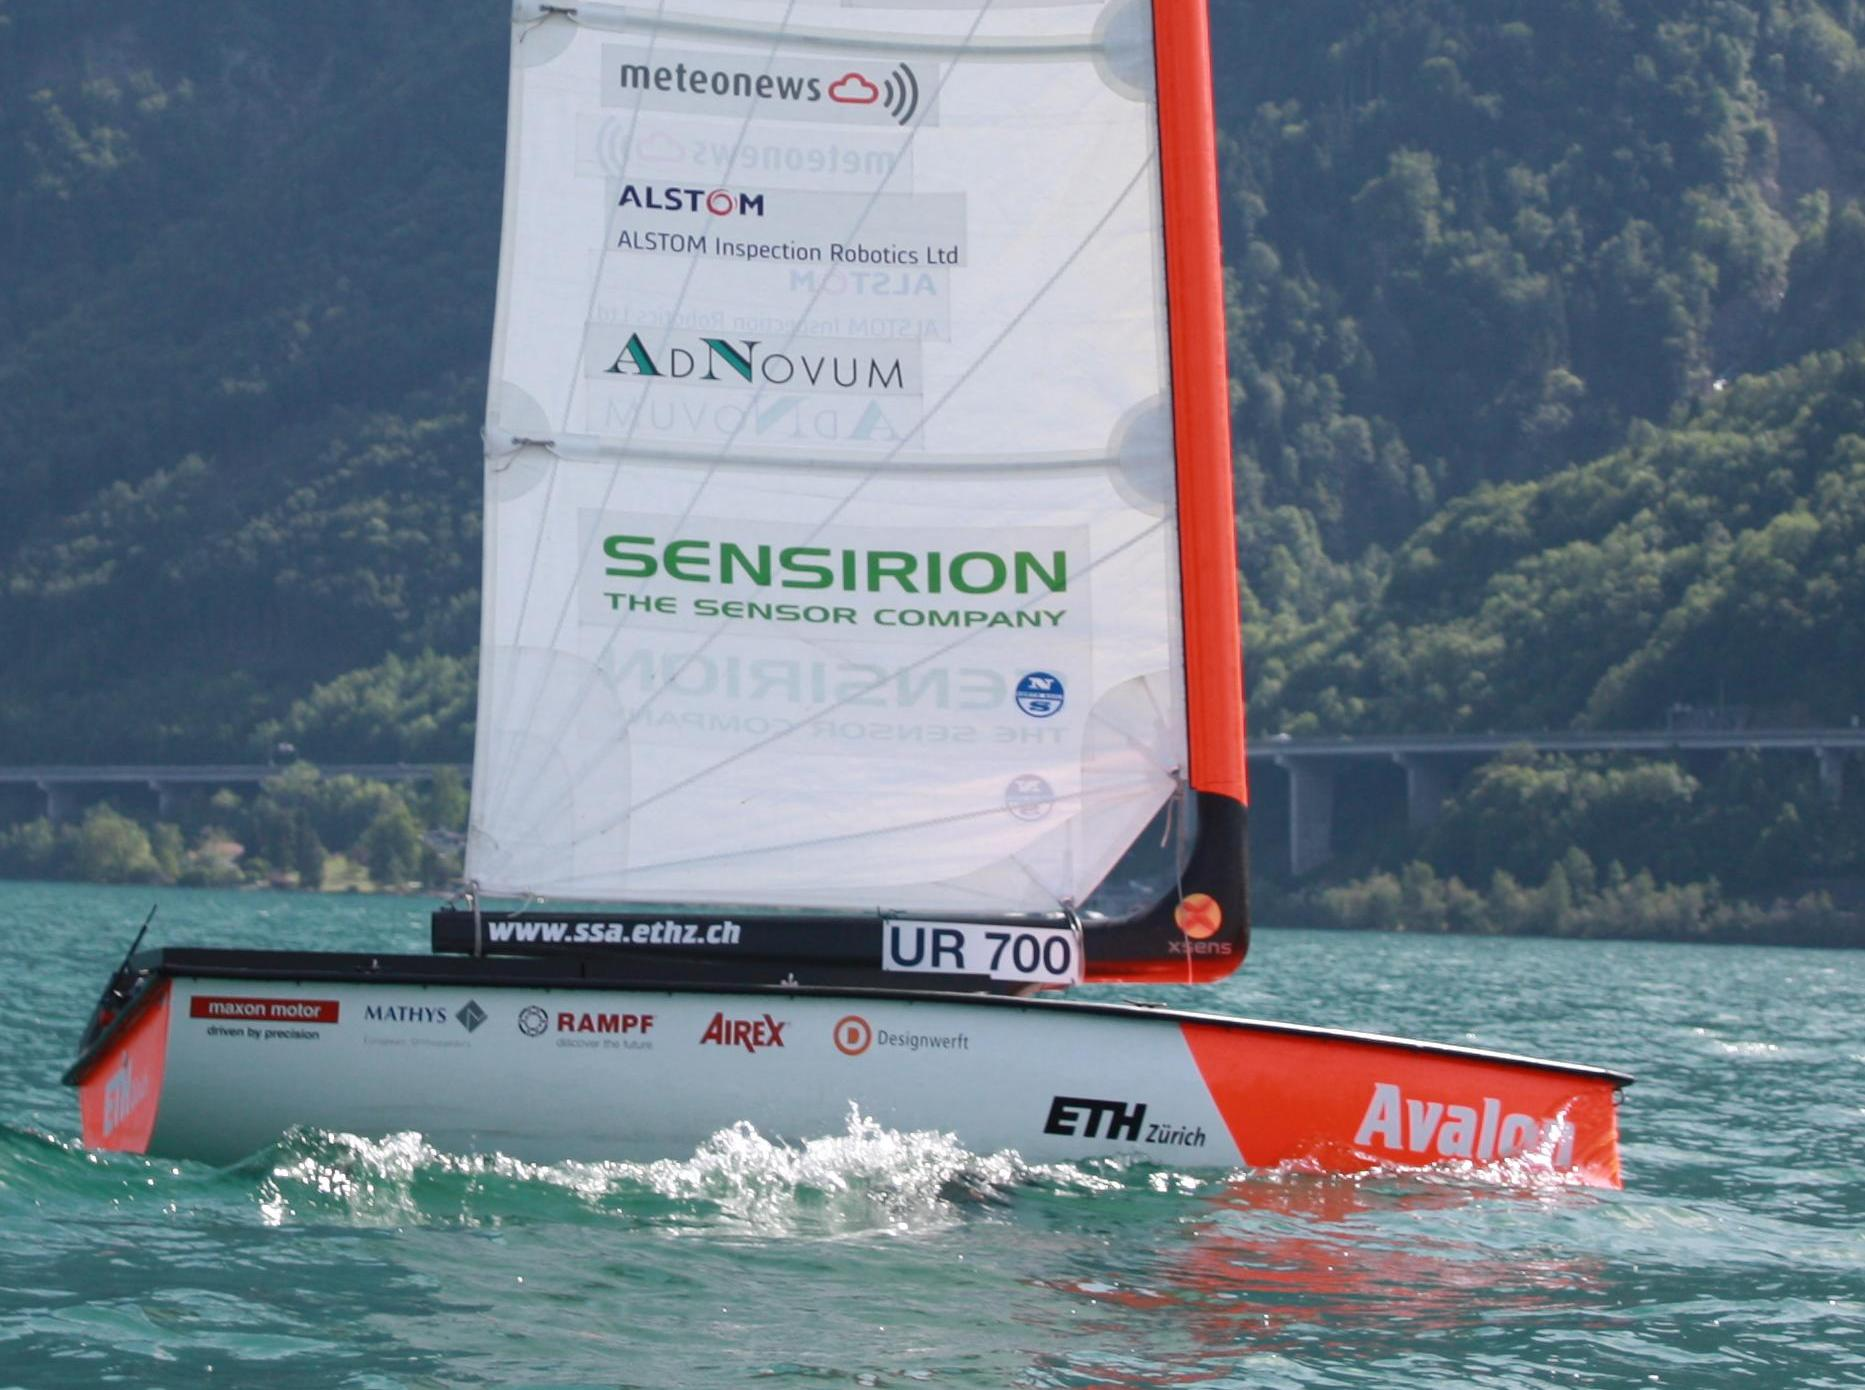
\includegraphics[width=0.75\columnwidth]{pics/IMG_0601_papercrop.jpeg}
\caption{Avalon during testing in high winds}
%\label{fig:avalon}
\end{figure}

\section{Conclusion and Outlook}
The proposed navigation and control software has been successfully implemented
in our autonomous sailboat \textsc{Avalon}. Several short-run tests both on
Swiss lakes and on the Atlantic Ocean have been carried out and have shown that the
described control and navigation system work. \textsc{Avalon} was exposed to
wind conditions ranging from almost 0 to 30 knots. The experimentally found
control parameters have proven to be well defined, keeping the vessel on course
even while sailing in rough sea states.

In very low wind speeds it was seen that the boat is able to sail much better
by itself than steered by us via remote control, because it is always aware of
the exact wind direction, even when human sailors hardly notice any wind at
all.

However, especially in reference to a possible crossing of the Atlantic Ocean,
several tests over a bigger period of time as well as longer distances have to
be performed in a next stage. 

By processing received AIS-signals, \textsc{Avalon} is able to identify other
ships in close proximity and therefore prevent collisions. However, small boats
that don't send position information cannot be recognized at this stage and
further research has to be done in identifying obstacles visually.   

Implementing a conventional and proved path planner like Dijkstra's for our
navigation system has proved well. Visually and analytically evaluated results
show that we achieve better solutions by taking the whole path into account
than by always optimising the heading at every current position. However, by
adding additional costs (like tunnel cost), optimal path solutions are not
always guaranteed.

Our goal for future work is to further optimise the software, especially
regarding energy consumption. For example a hysteresis could be added to the
sail tuner so that the sail does not constantly adapt to minor changes in wind
direction and speed. A further area of improvement could be in making use of
weather forecasts in the global navigation. For our boat this does not add much
value, because it is too slow to react to forecast weather changes.
